\chapter{Entwurf}

Nachdem in dem vorangegangenen Kapitel der aktuelle Stand des Formulars erläutert, sowie die Anforderungen zusammengetragen wurden, werden im folgendem Kapitel selbige Anforderungen in Kriterien umgewandelt und bewertet. Anhand dieser Kriterien werden mögliche Lösungsansätze verglichen. Somit wird ein optimaler Lösungsweg erarbeitet und in einem konkreten Plan zusammengefasst.

\section{Wahl der Technologie}
\label{ch:Techn}

Die Verwendung von Adobe Interactive Forms ist eine \ac{ABB} interne Vorgabe für diese Arbeit. Bis vor kurzem nutzte \ac{ABB} beziehungsweise die DE-IS nur Smart Forms im SAP.\footnote{Siehe Kapitel \ref{ch:Grundlagen}} Die Modernisierung beziehungsweise Digitalisierung von Geschäftsprozessen führt jedoch dazu, dass neue Anforderungen an die automatische Dokumentenerstellung gestellt werden\footnote{Siehe Kapitel \ref{ch:Ausblick}}. Diese Anforderungen kann Smart Forms in naher Zukunft nicht mehr erfüllen, da neue Entwicklungen seitens SAP SE hauptsächlich für die neuere Technologie, die Interactive Forms, entwickelt werden.

Ein weiterer Grund für den Technologiewechsel ist die Übersichtlichkeit der Inhalte. Die Aufspaltung in Schnittstelle und Formular bei den Interactive Forms führt dazu, dass das Layout getrennt von den Formularinhalten betrachtet beziehungsweise angepasst werden kann. 

Aufgrund dieser begründeten Vorgabe findet keine weitere Auswahl beziehungsweise Bewertung von alternativen Technologien statt.


\section{Bewertung der Lösungsansätze}
\label{ch:Bewertung}

Oftmals sind mehrere Lösungsansätze für spezifische Probleme möglich. Um diese miteinander zu vergleichen, wurde in Abbildung \ref{figNutz} eine Gewichtung, der in Kapitel \ref{ch:Anf} beschriebenen Anforderungen, durchgeführt\footnote{Diese Gewichtung fand in Zusammenarbeit mit dem Leiter des GTS-Modul der DE-IS statt}. 

\begin{figure}[ht]
	\centering
	\makebox[\textwidth][c]{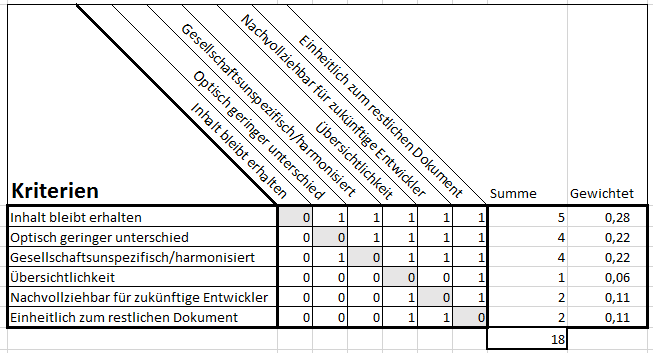
\includegraphics[width=1\textwidth]{img/Nutzwert.png}}%		
	\caption{Nutzwertanalyse der Anforderungen}
	\label{figNutz}
\end{figure}

Diese Gewichtung kann verwendet werden, um eine Wahl zwischen Lösungsalternativen zu treffen. Es ist erkennbar, dass vor allem inhaltliche und optische Unterschiede vermieden werden müssen. Es muss ein Kompromiss zwischen der technischen Übersichtlichkeit und der Erfüllung der Anforderungen des neuen Formulars gefunden werden.


\section{Automatische Migration}
\label{ch:Migration}

Marcel Schmiechen beschreibt in seinem Buch über Interaktive Formulare im SAP \footcite{Schmiechen.2016} in Kapitel 8.4 das automatische Migrationsverfahren im SAP-Standard im Vergleich zu einer Neuentwicklung als nicht lohnenswert\footnote{Vgl. \cite{Schmiechen.2016} S.189}. Dieses Verfahren bietet die Möglichkeit in kürzester Zeit ein Smart Forms-Formular in ein Interactive Adobe \ac{PDF} umzuwandeln. Jedoch kommt es gerade bei größeren Dokumenten zu Fehlern bei der Migration. Dies hat auch der Test anhand der \ac{LLE} bestätigt. Die Schnittstelle konnte fehlerfrei übernommen werden, jedoch führte die Migration zu großen Fehlern in dem Formularteil. In Abbildung \ref{Migration} ist zu sehen, dass teilweise Attribute von Elementen nicht befüllt werden konnten. In diesem Fall fehlte vor allem das Absenderland für die verwendeten Addressknoten. Zusätzlich führten lange Namen von Elementen der Smart Form zu weiteren Fehlern, da die maximale Namenslänge bei den Interactive Forms zu lange Namen abschneidet. Daraus resultiert, dass Elemente gleich benannt sind.

Um das Layout zu überprüfen, musste das Formular zunächst überarbeitet werden, sodass die Fehlermeldungen nicht mehr die Aktivierung des Dokumentes verhindern. Nachdem die nötigen Änderungen durchgeführt wurden, konnte das Layout überprüft werden. 
\begin{figure}[ht]
	\centering
	\makebox[\textwidth][c]{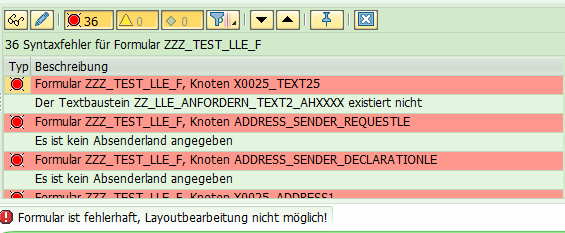
\includegraphics[width=1\textwidth]{img/Migration_Test.png}}%		
	\caption{Fehler bei der Migration der \acs{LLE}}
	\label{Migration}
\end{figure}

Zu Beginn wurde der Aufbau des Dokumentes überprüft. Für jede nötige Seite der \ac{LLE} war eine Masterseite vorhanden, jedoch nur für zwei Seiten auch eine Inhaltsseite. Das hat zur Folge, dass bei der Verwendung dieses Formulars nur diese beiden Seiten ausgedruckt werden würden. Unabhängig vom Aufbau und Inhalt des migrierten Formulars konnten noch weitere technische Fehler gefunden werden. Ein schwerwiegendes Problem ist, dass jedes Feld mit dynamischem Inhalt nur über den Namen mit dem zugehörigen Datensatz verbunden ist. Diese Zuordnung funktioniert zwar, jedoch ist sie sehr fehleranfällig bei Namensänderungen beziehungsweise neuen Zuordnungen, da so an mehreren Stellen die Änderungen vorgenommen werden müssen. In Abbildung \ref{Namen-Fehler} ist zu sehen, dass SAP diese Elemente mit einer Warnung versehen hat.



Neben der Struktur und den Datenbindungen kam es auch bei anderen Funktionen zu Fehlern bei der Migration. Die Tabelle konnte nicht in einer verwendbaren Weise übertragen werden und Texte, welche über Bedingungen in mehreren Sprachen vorhanden waren, wurden untereinander angezeigt. Da der Aufwand für die Überarbeitung dieser ganzen Fehler sehr hoch ist, vor allem wenn eine Harmonisierung beziehungsweise Optimierung der Inhalte stattfinden soll, wird von dieser Weise der Migration des Formularteils abgesehen. Da die migrierte Schnittstelle keine Fehler aufwies kann sie für das neue Formular verwendet werden. Auf Grund der Tatsache das die selben Daten benötigt werden sind auch weitere Anpassungen nicht nötig.
\begin{figure}[ht]
	\centering
	\makebox[\textwidth][c]{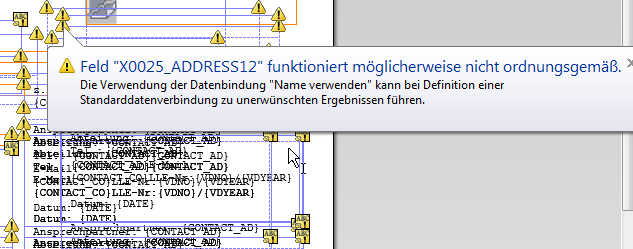
\includegraphics[width=1\textwidth]{img/Namen-Fehler.png}}%		
	\caption{Warnung bei der Verwendung von "Namen verwenden"}
	\label{Namen-Fehler}
\end{figure}

\section{Schnittstelle}

In der Schnittstelle werden die Inhalte des Formulars, welche aus dem SAP System stammen, definiert, sowie weitere benötigte Strukturen festgelegt.\footnote{Siehe Kapitel \ref{ch:Schnittstelle}}
Die tatsächlichen Inhalte der \ac{LLE} bleiben gleich, egal welche Technologie benutzt wird. Somit kann die Schnittstelle aus der Formularschnittstelle des Smart Forms-Formular abgeleitet werden. Für die Erstellung der Schnittstelle kann daher die SAP-Standard-Migration verwendet werden.\footnote{Siehe Kapitel \ref{ch:Migration}}


\section{Formular}

\subsection{Allgemein}

Für das Anschreiben der ABB muss eine Seite im Layout-Bereich des Formulars erstellt werden. Die Inhalte des Anschreibens sind in den folgenden Kapiteln erläutert. Allgemein muss die Schriftart und Schriftgröße aus dem Smart Forms-Formular übernommen werden. Bezüglich der Benennung der verschiedenen Objekte und Elemente gilt es sprechende, erklärende und eindeutige Namen zu verwenden. Um die dynamischen Inhalte in den statischen Text des Anschreibens einzufügen, werden Fließtextfelder benutzt\footnote{Siehe Kapitel \ref{ch:Aufbau}}\footnote{Vgl. \cite{Hauser.2015} S. 319}.

\subsection{Anschreiben - Logos}

In Kapitel \ref{ist_logos} wurde festgestellt, dass Logos weiterhin gesellschaftsspezifisch verwendet werden müssen. Dementsprechend muss für jedes der sechs Logos ein eigenes Grafik-Element im Kontext-Bereich angelegt sowie im Layout-Bereich positioniert werden. Für die dynamische Anzeige der Logos werden diese Elemente mit einer Bedingung, welche die \ac{AH}-Nummer abprüft, versehen. Die tatsächlichen Logos werden, wie auch in Smart Forms, über den Namen des "`GRAPHICS"' Objektes eingebunden. Im Layout-Bereich werden die Logos als Bildfelder eingefügt und - kongruent zum alten Formular - positioniert. 

\subsection{Anschreiben - Adressköpfe}

Eine automatische Darstellung von Adressen ist im gleichen Sinne bei Interactive Forms möglich. Hierzu wird ebenfalls eine Adressnummer benötigt und zusätzlich das Land des Absenders\footnote{Siehe Kapitel \ref{Migration}}.

Die Position der Adressfelder ist im Smart Forms-Formular nicht standardisiert und nicht allgemein für alle Gesellschaften gleich. Für das neue Formular soll die Position gleich für alle Gesellschaften sein, um möglichst wenige verschiedene Elemente im Formular zu haben. Für die Festlegung der Ausrichtung der Empfängeradresse wird ein Standard-Briefumschlag mit Fenster als Referenz hinzugezogen. Somit wird der Versand der \ac{LLE} per Post vereinfacht, ohne das jetzige Layout des Dokumentes zu beeinträchtigen. Der Adressblock des Empfängers sowie die schmale Variante des Absenders kann in einem Element zusammengefasst werden. Um die unterschiedliche Formatierung innerhalb des Elementes nutzen zu können, wird von einem automatischen Adressblock abgesehen. Stattdessen wird die Adresse mit Hilfe dynamischer Felder im Fließtext dargestellt. Der Vorteil dieser Variante ist es, dass nur ein Element für alle Gesellschaften verwendet werden kann, aber trotzdem variable Inhalte möglich sind.
 Würde stattdessen ein automatisches Adressfeld verwendet werden, müssten mehrere Elemente angelegt und positioniert werden um verschiedene Formatierungen der Inhalte beizubehalten.
 
Für die Adressdaten der Absendergesellschaft auf der rechten Seite des Anschreibens kann ein automatisch erstelltes Adresselement eingesetzt werden. Hierfür muss lediglich ein Element im Layout-Bereich hinzugefügt werden, welches auf das Adresselement im Kontextbereich referenziert. Die Definition dieses Elements kann hierbei aus dem Smart Forms-Formular übernommen werden. Über eine Bedingung wird dieses Feld anschließend für die \ac{AH} 2000 \footnote{Siehe Kapitel \ref{ist:adr}} ausgeblendet.

Die Kontaktdaten des Mitarbeiters werden ebenfalls mit Hilfe von Feldern im Fließtext dargestellt, da nicht alle benötigten Informationen Adressdaten sind, welche über einen Adressenbaustein eingefügt werden können. Hierfür wird ein weiteres Element benötigt, womit die Adressen mit drei Elementen vollständig wären. Dieses letzte Element wird inhaltlich und bedingungslos für alle Gesellschaften verwendet.

\subsection{Anschreiben - Sonstige Inhalte}

Das in Kapitel \ref{ist:rueck} erläuterte Info-Feld sowie die Fußzeilen müssen ebenfalls in das neue Formular übertragen werden. Für die Umsetzung gibt es zwei Möglichkeiten:

\subsubsection{Text als Feld im Fließtext}

Indem der anzuzeigende Text in einer Variable in der Schnittstelle eingefügt wird, kann der Text über ein Feld im Fließtext angezeigt werden. Hierfür ist es erforderlich, dass sowohl die Schnittstelle also auch das Formular angepasst werden, da der Text zunächst erst in einer Variable abgespeichert werden muss. Sollten Änderungen am Text nötig sein, müssten somit an mehreren Stellen Anpassungen vorgenommen werden. Dies steht nicht im Sinne der Optimierung des Formulars. Des Weiteren ist eine Formatierung des anzuzeigenden Textes nicht möglich, da in einer Variable nur reiner Text ohne Absatz und Schriftformatierung abgespeichert werden kann.

\subsubsection{Textbaustein}

Der Inhalt wird als Textbaustein angelegt, welcher für die relevanten Gesellschaften eingelesen werden kann. Die bedingte Anzeige ist somit ersichtlich und der Text an einer genauen Stelle für eventuell nötige Anpassungen verfügbar.
Diese Methode steht im Sinne der definierten Anforderungen\footnote{Siehe Kapitel \ref{ch:Bewertung}} und wird somit verwendet. 

\subsection{Anschreiben der \acs{LLE}}

Für das Anschreiben der \ac{LLE} muss zunächst eine Seite erstellt werden, welche in die Seitenzählung miteinbezogen wird. Der Text des Anschreibens kann aus dem Smart Forms-Formular übernommen werden\footnote{Siehe Kapitel \ref{ist:le}}. Hierfür ist ein Textfeld notwendig, welches mit Hilfe von Felder im Fließtext mit dynamischen Inhalten, beispielsweise Angaben zum Gültigkeitszeitraum, erweitert wird. 

\subsection{Materialliste}

Für Seiten der Materialliste sind mehrere Schritte zu beachten. Zunächst gilt es die Seite, abgesehen von der tatsächlichen Liste, zu erstellen. Für die Adressdaten sowie die Verwaltungseinheit werden Felder im Fließtext verwendet. Diese Kopfdaten werden über der Liste angeordnet, konvergent zum Smart Forms-Formular. Anschließend muss die Materialliste erstellt werden. Hierfür muss zunächst, ähnlich wie bei Smart Forms, eine Schleife im Kontextbereich des Formulars definiert werden. Über diese Schleife ist es möglich, die einzelnen Zeilen der Materialliste im Formular anzuzeigen. Im Layoutbereich wird anschließend die Liste mit einer Kopfzeile  erstellt, welche die Spaltenbezeichnungen beinhaltet. Abschließend muss die Seite der Materialliste in einer Weise konfiguriert werden, dass bei einer längeren Liste die Tabelle auf die nächste Seite umgebrochen wird. Hierbei darf kein Umbruch innerhalb einer Zeile möglich sein. Zudem muss jede benötigte Folgeseite ebenfalls die Kopfdaten sowie die Kopfzeile der Materialliste darstellen. Ein Element für die Anzeige der Seitenanzahl wird am unteren Ende der Seite eingefügt. Nach der letzten Listenseite muss die anschließende Formularseite eingefügt werden.

\subsection{Legende}
Die letzte Seite des Formulars beinhaltet die Legende\footnote{Siehe Kapitel \ref{ist:leg}}.
Die Legende ist ein statischer Text und für alle Gesellschaften gleich. Daher wird der Text als Textbaustein in das Formular eingebunden, da so Änderungen zentral vorgenommen werden können. Eine Alternative zu dem Textbaustein wäre es, den Text direkt in das Formular durch ein Textfeld zu schreiben. Dies würde dazu führen, dass für jede Änderung das Formular bearbeitet werden muss. Der Textbaustein dagegen kann sehr schnell angepasst werden.



\section{Customizing}

Nachdem das Formular erstellt wurde, wird es im Customizing jeder Gesellschaft zugeordnet\footnote{Siehe Kapitel \ref{ch:ist-aufbau}}. Somit ist die technische Umstellung auf das neue Formular abgeschlossen.



%\section{Dokumentation}

%Um zukünftige Bearbeitung der PDF zu vereinfachen wird eine Dokumentation nötig sein. Hier wird der fachliche Hintergrund des Dokumentes erläutert sowie die technische Umsetzung dokumentiert. Erklärungen von komplizierten Inhalten sowie generelle Informationen zur Umsetzung der \ac{LLE} werden ebenfalls in der Dokumentation festgehalten. 

%Es ist nur sinnvoll die Dokumentation direkt an das Formular anzufügen in SAP. In der Transaktion SFP kann zu einem Formular eine Dokumentation hinterlegt werden. Diese ist standardmäßig unterteilt in folgende Unterpunkte:

%\begin{itemize}
%	\item Verwendung
%	\item Einschränkungen
%	\item Aufruf
%	\item Kontext
%	\item Layout
%	\item Weitere Hinweise
	
%\end{itemize}

%Mit Hilfe dieser Unterteilung wird das neue Formular beschrieben und erläutert.